\section{Hyperobjects: The Building Blocks of the New Internet}

Simply put, hyperobjects are game assets such as avatars, items, and game environments that can be used across different games, chains, worlds, platforms, marketplaces, and connected IRL experiences, that form the foundation of in-game economies and interactions.

Hyperobjects share similarities with NFTs, but because of the scalability afforded by AO, an individual hyperobject can be a large application, such as a AAA game or AI agent, as opposed to a simple image. Players and creators can use hyperobjects to craft unique experiences, build new worlds, and participate in shared economies. Commonly used file types used for gaming, such as VRMs \cite{VRM2024}, GLBs, OBJs and USDZs\footnote{These file formats serve different purposes in 3D gaming and virtual worlds: VRM is optimized for humanoid avatars with standardized rigging, GLB/OBJ are general-purpose 3D model formats supporting meshes and textures, and USDZ is Apple's AR-optimized format. This diversity of formats enables hyperobjects to be compatible with a wide range of platforms and use cases.}, can be used as hyperobjects. Designed for interoperability, flexibility, and permanence, hyperobjects can be thought of as the hypertext of the gaming world in that they function as connective tissue---flexible, transferable, and useful across multiple platforms -- much like hypertext in the Internet we use today.

\subsection{Categories of Hyperobjects}

\subsubsection{Avatars (``Action Figures'')}
Action Figures serve as players' digital identities, representing their presence, abilities, and progression across different virtual worlds. These avatars are designed for full interoperability, functioning seamlessly across multiple games, social platforms, and streaming services while maintaining their skills, achievements, and personalized characteristics. 

Players can continuously evolve their Action Figures through customization and upgrades using other Hyperobjects, creating a persistent digital identity that spans the entire ecosystem.

\subsubsection{Game Assets (``Action Items'')}
Action Items are digital objects designed for use within games and virtual worlds. These items come in two main varieties, as illustrated in Figures \ref{fig:consumable_items} and \ref{fig:durable_items}: consumable items are one-time-use objects like power-ups, health packs, or crafting materials that are depleted upon use, while durable items are persistent assets such as weapons, tools, or collectibles that remain in the player's inventory and can be traded, upgraded, or staked over time.


\begin{figure}[t]
\centering
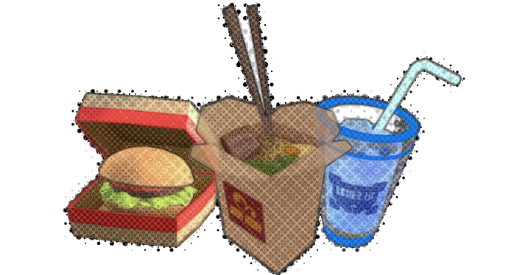
\includegraphics[width=0.9\columnwidth]{images/image4.png}
\vspace{1em}
\caption{Consumable Hyperobject: Action Items from the Basejump gaming platform boost an Action Figure's health when consumed, and can be used as melee weapons or projectiles in battle.}
\label{fig:consumable_items}
\end{figure} 



\begin{figure}[t]
\centering
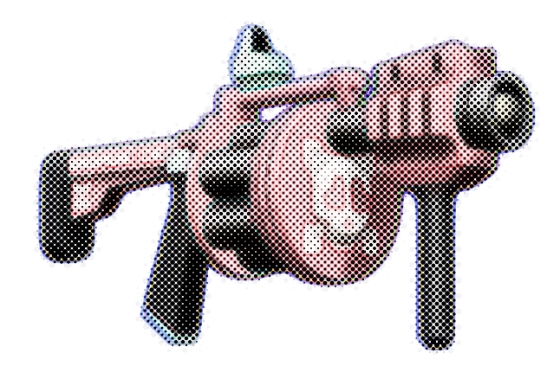
\includegraphics[width=0.8\columnwidth]{images/image5.png}
\vspace{1em}
\caption{Durable Hyperobject: An Action Item from the Basejump gaming platform (the EMP Glo-Stick Rocket Launcher) that exhibits context-dependent behavior: If used in web3 game Nifty Island, it fires bullets. In the battle game on Basejump, it fires glo-sticks.}
\label{fig:durable_items}
\end{figure}


\subsubsection{Game Environments (``Worlds'')}
\begin{itemize}
\item Maps, levels, and immersive environments that define the setting and rules of gameplay
\item Creators can publish and register Worlds using the Action substrate, ensuring interoperability with other assets
\end{itemize}

\subsection{Context-Dependent Behavior}

Hyperobjects exhibit \textbf{context-dependent behavior}, dynamically adapting to the specific game or world in which they are used. This ensures:

\begin{itemize}
\item \textbf{Defaults-first design}\footnote{Defaults-first design means hyperobjects come with pre-configured, sensible behaviors that work immediately in any compatible environment. This approach significantly reduces integration complexity for developers and ensures a consistent baseline experience, while still allowing for customization when needed.}: Hyperobjects ``just work'' in all environments with robust defaults, reducing onboarding friction
\item Developers can override or extend functionality through the Hyperobject Registry, introducing unique mechanics while maintaining interoperability
\end{itemize}

For example, the the Mutatio Fly (Figure \ref{fig:mutatio_fly}) is a piece of digital art that was turned into a drone Hyperobject in Basejump, allowing players to use it as a flying companion in the game

\begin{figure}[t]
  \centering
  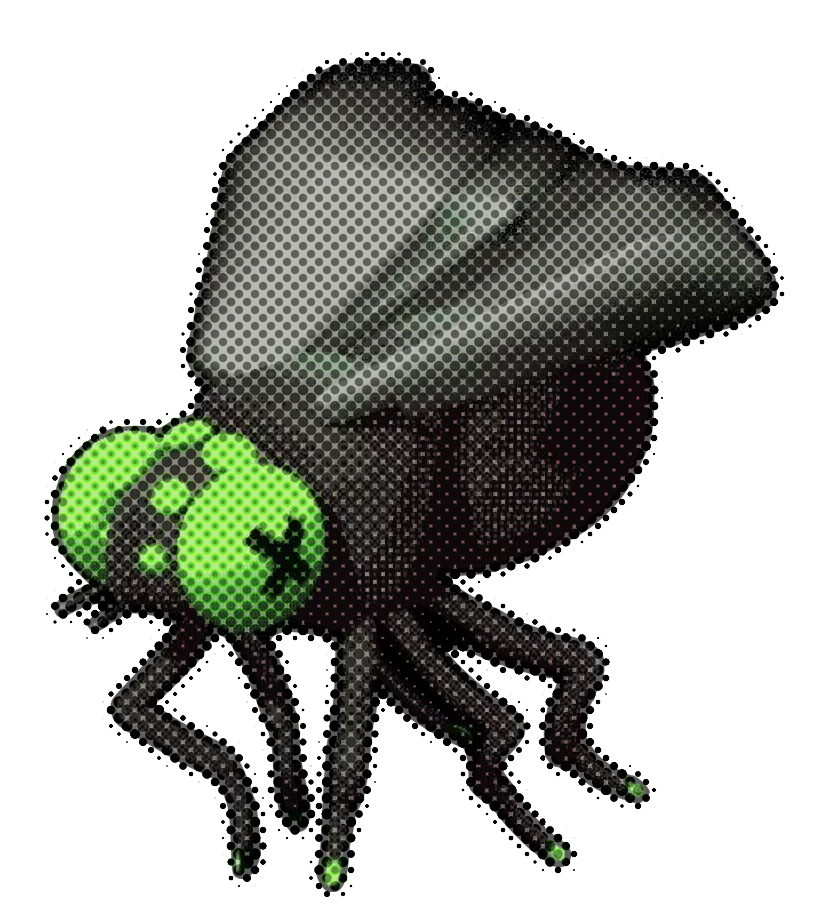
\includegraphics[width=0.7\columnwidth]{images/image5b.png}
  \vspace{1em}
  \caption{Giving existing game assets new utility as  Hyperobjects: Mutatio Flies released in Spring 2024 by XCOPY and Neon Glitch were given new utility in Basejump Winter 2024, where they can now also be used as drones that Action Figures can equip and use in the Basejump platform.}
  \label{fig:mutatio_fly}
\end{figure}
  
\begin{figure}
\centering
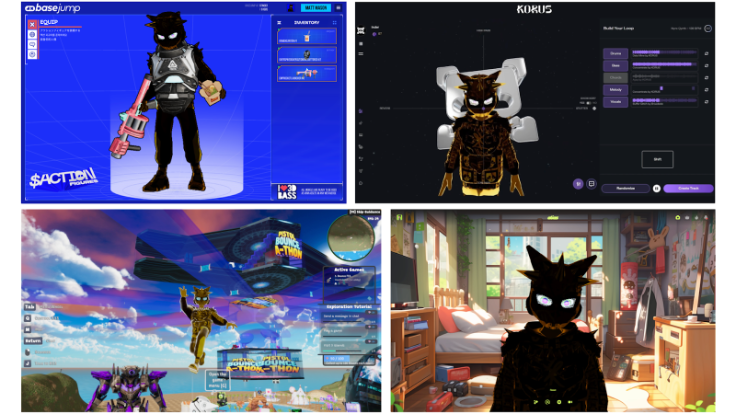
\includegraphics[width=\columnwidth]{images/image6.png}
\caption{An Action Figure hyperobject (Broadside OG 2969 - Stinger) exhibits context-dependent behavior in different platforms. Top Left: Stinger equipping EMP Glo-Stick Rocket Launcher and Ramen Action Items on Basejump. Top Right: Stinger working as a music-making companion in the AI music platform Korus. Bottom Left: Stinger functioning as a player avatar in Nifty Island. Bottom Right: Stinger performing as a live webcam avatar for 'v-tubing' in the Alias streaming video application.}
\label{fig:context_dependent}
\end{figure}

\subsection{Implementation}

The hyperobject design takes inspiration from some of the EVM ecosystem's primitives, such as the traditional ERC-721 (non-fungible) \cite{Entriken2018} and ERC-1155 (semi-fungible) \cite{Radomski2018} tokens, as well as newer standards like ERC-6551 (token-bound accounts) \cite{Windle2023}. The Action substrate also takes cues from other gaming protocols on EVM and elsewhere, such as Enjin \cite{Blagov2023}, Open Meta \cite{Gill2024}, Axie Infinity \cite{Nguyen2020}, and Immutable X \cite{Ferguson2021} among others. However, hyperobjects leverage AO's decentralized computer architecture, with each unique hyperobject running as a unique AO process with corresponding Arweave data representing its underlying assets. \cite{AtomicAsset}

The Hyperobject interface adheres to the AO community's developing process and token standards, including Atomic Assets \cite{AtomicAssetsSpec2024}, ANS-110 \cite{ANS110_2024} and ANS-103 \cite{ANS103_2024}. Figure \ref{fig:hyperobject_interface} shows the core interface methods that every Hyperobject implements.

\begin{figure}[t]
\begin{lstlisting}[basicstyle=\ttfamily\small]
-- Get info about the HyperObject process
Info() -> {
  Name, Creator, Metadata
}

-- Get balance of a specific account
Balance(Target?) -> {
  Balance, Ticker, Account, Data
}

-- Get all account balances
Balances() -> {
  Data -- JSON-encoded map
}

-- Get total supply of the Hyperobject
Total-Supply() -> {
  Action, Data, Ticker
}

-- Emits standard Credit-Notice and Debit-Notice
Transfer(Recipient, Quantity)

-- Callable only by the Hyperobject owner process
Mint(Quantity: string)

-- Callable only by a holder of the Hyperobject
Burn(Quantity: string)
\end{lstlisting}
\caption{Hyperobject Handler Interfaces (pseudocode): Core methods for querying state and performing transactions in the Hyperobject protocol.}
\label{fig:hyperobject_interface}
\end{figure}
